\documentclass{beamer}

\mode<presentation>
{
  \usetheme{CambridgeUS}
  \setbeamercovered{transparent}
}

\usepackage[english]{babel}
\usepackage[latin1]{inputenc}
\usepackage{times}
\usepackage[T1]{fontenc} 
% Or whatever. Note that the encoding and the font should match. If T1
% does not look nice, try deleting the line with the fontenc.
\usepackage{amsmath}

\newcommand{\linespace}{\vskip 0.25cm}

\definecolor{MyForestGreen}{rgb}{0,0.7,0} 
\newcommand{\tableemph}[1]{{#1}}
\newcommand{\tablewin}[1]{\tableemph{#1}}
\newcommand{\tablemid}[1]{\tableemph{#1}}
\newcommand{\tablelose}[1]{\tableemph{#1}}

\definecolor{MyLightGray}{rgb}{0.6,0.6,0.6}
\newcommand{\tabletie}[1]{\color{MyLightGray} {#1}}

% The text in square brackets is the short version of your title and will be used in the
% header/footer depending on your theme.
\title[Test-First vs. Test-Last Testing]{An Exploration into the Current State \\ of Test-First vs. Test-Last Testing}

% Sub-titles are optional - uncomment and edit the next line if you want one.
% \subtitle{Why does sub-tree crossover work?} 

% The text in square brackets is the short version of your name(s) and will be used in the
% header/footer depending on your theme.
\author[Thomas]{Christopher Morris Thomas}

% The text in square brackets is the short version of your institution and will be used in the
% header/footer depending on your theme.
\institute[U of Minn, Morris]
{
  Division of Science and Mathematics \\
  University of Minnesota, Morris \\
  Morris, Minnesota, USA
}

% The text in square brackets is the short version of the date if you need that.
\date[2013 Fall Senior Seminar] % (optional)
{2013 Fall Senior Seminar}

% Delete this, if you do not want the table of contents to pop up at
% the beginning of each subsection:
\AtBeginSection[]
{
  \begin{frame}<beamer>
    \frametitle{Outline}
    \tableofcontents[currentsection, hideothersubsections]
  \end{frame}
}

\begin{document}

\begin{frame}
  \titlepage
\end{frame}

% For a 20-25 minute senior seminar talk you probably want something like:
% - Two or three major sections (other than the summary).
% - At *most* three subsections per section.
% - Talk about 30s to 2min per frame. So there should probably be between
%   15 and 30 frames, all told.

\section*{Overview}

\subsection*{The big picture}

\begin{frame}
  \frametitle{The big picture}
  
  \begin{columns}
  \begin{column}{0.6\textwidth}
  \begin{itemize}
  	\item Developmental plasticity: a powerful source of flexibility in biology
	\item Most EC \& GP systems don't have a developmental phase
	\item Even fewer allow for plasticity during development
	\item N-gram GP has natural developmental phase
	\item Can we add plasticity?
  \end{itemize}
  \end{column}
  \begin{column}{0.4\textwidth}
   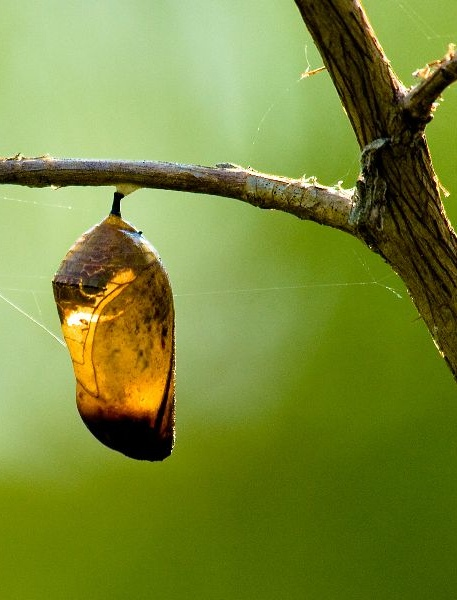
\includegraphics[width=0.95\textwidth]{Illustrations/Empty_cocoon_crop_by_Bluedrakon_from_Flickr.jpg}
       \\
    \only{\tiny{Bluedrakon \\ \url{http://tr.im/pWUi} }}
  \end{column}
  \end{columns}
\end{frame}

\subsection*{Outline}

\begin{frame}
  \frametitle{Outline}
  \tableofcontents[hideallsubsections]
\end{frame}

\section[Background]{Background}
\subsection{What is testing?}

\begin{frame}
\frametitle{Software Testing Defined}
\end{frame}

\subsection{Test-Last Testing and Waterfall Development}

\begin{frame}
\frametitle{Waterfall Development}
\end{frame}

\begin{frame}
\frametitle{Test-Last Testing}
\end{frame}

\subsection{Test-First Testing and Test Driven Development}

\begin{frame}
\frametitle{Agile Software Development}
\end{frame}

\begin{frame}
\frametitle{Test Driven Development}
\end{frame}

\begin{frame}
\frametitle{Test-First Testing}
\end{frame}

\section[Comparison of Testing Methods]{Comparison Between Test-First and Test-Last Testing}

\subsection{Perception of Test-First vs Test-Last}

\begin{frame}
\frametitle{Perceptions from a Pro Test-First User}
\end{frame}

\begin{frame}
\frametitle{Perceptions from a Pro Test Last User}
\end{frame}


\subsection{Current Data}

\begin{frame}
\frametitle{Study by Kollanus}
\end{frame}

\begin{frame}
\frametitle{Test-First vs Test Last Study}
In 2012 Lemos et al preformed an experiment comparing test-first and test-last testing with auxiliary functions (10-200 lines of code).

\linespace

In the study, Lemos had 39 third year computer science students with basic test-first and test-last knowledge solve coding problems using test-first or test-last development methodologies.

\linespace

After the study was completed Lemos found that Test-First testing:
	\begin{itemize}
		\item produced 40\% more code coverage than test-last testing
		\item took 12\% longer to implement then test-last testing 
		\item Did not produce more effective code quality
	\end{itemize}
\end{frame}

\subsection{Discussion}

\begin{frame}
\frametitle{Contradictory Studies}
\end{frame}

\begin{frame}
\frametitle{Conclusions}
\end{frame}

\section[Different Implementations of Test-First]{Different ways of Implementing Test-First Testing} 
\subsection{The challenges of Test Driven Development}
\begin{frame}
\frametitle{Difficulty of TDD}
\end{frame}
\subsection{Behavior Driven Development}
\begin{frame}
\frametitle{Behavior Driven Development (BDD)}
\end{frame}


\section[Summary]{Summary}
\begin{frame}
\frametitle{Conclusions}
\end{frame}


\end{document}


